% mnras_template.tex
%
% LaTeX template for creating an MNRAS paper
%
% v3.0 released 14 May 2015
% (version numbers match those of mnras.cls)
%
% Copyright (C) Royal Astronomical Society 2015
% Authors:
% Keith T. Smith (Royal Astronomical Society)

% Change log
%
% v3.0 May 2015
%    Renamed to match the new package name
%    Version number matches mnras.cls
%    A few minor tweaks to wording
% v1.0 September 2013
%    Beta testing only - never publicly released
%    First version: a simple (ish) template for creating an MNRAS paper

%%%%%%%%%%%%%%%%%%%%%%%%%%%%%%%%%%%%%%%%%%%%%%%%%%
% Basic setup. Most papers should leave these options alone.
\documentclass[a4paper,fleqn,usenatbib]{../mnras}

% MNRAS is set in Times font. If you don't have this installed (most LaTeX
% installations will be fine) or prefer the old Computer Modern fonts, comment
% out the following line
\usepackage{newtxtext,newtxmath}
% Depending on your LaTeX fonts installation, you might get better results with one of these:
%\usepackage{mathptmx}
%\usepackage{txfonts}

% Use vector fonts, so it zooms properly in on-screen viewing software
% Don't change these lines unless you know what you are doing
\usepackage[T1]{fontenc}
\usepackage{ae,aecompl}


%%%%% AUTHORS - PLACE YOUR OWN PACKAGES HERE %%%%%

% Only include extra packages if you really need them. Common packages are:
\usepackage{graphicx}	% Including figure files
\usepackage{amsmath}	% Advanced maths commands
\usepackage{amssymb}	% Extra maths symbols
\usepackage[flushleft]{threeparttable} % For table notes

%%%%%%%%%%%%%%%%%%%%%%%%%%%%%%%%%%%%%%%%%%%%%%%%%%

%%%%% AUTHORS - PLACE YOUR OWN COMMANDS HERE %%%%%

% Please keep new commands to a minimum, and use \newcommand not \def to avoid
% overwriting existing commands. Example:
%\newcommand{\pcm}{\,cm$^{-2}$}	% per cm-squared
\newcommand{\Nant}{N_{\text{ant}}} 
\newcommand{\Npix}{N_{\text{pix}}}
\newcommand{\dif}{\mathrm{d}}

%%%%%%%%%%%%%%%%%%%%%%%%%%%%%%%%%%%%%%%%%%%%%%%%%%

%%%%%%%%%%%%%%%%%%% TITLE PAGE %%%%%%%%%%%%%%%%%%%

% Title of the paper, and the short title which is used in the headers.
% Keep the title short and informative.
\title[E-field Parallel Imaging Correlator]{A Generic and Efficient E-field Parallel Imaging Correlator for Next-Generation Radio Telescopes}

% The list of authors, and the short list which is used in the headers.
% If you need two or more lines of authors, add an extra line using \newauthor
\author[Thyagarajan et al.]{
Nithyanandan Thyagarajan,$^{1}$\thanks{E-mail: t\_nithyanandan@asu.edu}
Adam P. Beardsley,$^{1}$
Judd D. Bowman$^{1}$
\newauthor
and Miguel F. Morales$^{2}$
\\
% List of institutions
$^{1}$Arizona State University, School of Earth and Space Exploration, Tempe, AZ 85287, USA\\
$^{2}$University of Washington, Department of Physics, Seattle, WA 98195, USA\\
}

% These dates will be filled out by the publisher
\date{Accepted XXX. Received YYY; in original form ZZZ}

% Enter the current year, for the copyright statements etc.
\pubyear{2015}

% Don't change these lines
\begin{document}
\label{firstpage}
\pagerange{\pageref{firstpage}--\pageref{lastpage}}
\maketitle

% Abstract of the paper
\begin{abstract}
Modern radio telescopes are favouring densely packed array layouts 
consisting of a large number of antennas 
($N_\textrm{a}\gtrsim 1000$--$\gtrsim 10000$). Since the cost of traditional 
correlators scales as $\mathcal{O}(N_\textrm{a}^2)$, there will be a steep cost for 
realizing the full imaging potential of these powerful instruments. Through 
our generic and efficient E-field Parallel Imaging Correlator (EPIC), we present 
the first software demonstration of a generalized direct imaging algorithm 
known as the Modular Optimal Frequency Fourier (MOFF) imager. It takes 
advantage of the multiplication-convolution theorem of Fourier transforms. Not 
only does it bring down the cost to $\mathcal{O}(N_\textrm{a}\log N_\textrm{a})$ 
but can also image from irregularly arranged heterogeneous antenna arrays. 
EPIC is highly modular and parallelizable. It is implemented in object oriented 
Python and is publicly available. We have verified the images produced to be 
mathematically identical to those produced using traditional techniques. We have 
also validated our implementation on data observed with the Long Wavelength 
Array. Antenna systems with a dense filling factor consisting of a large number 
of antennas such as LWA, SKA, and HERA will gain a significant advantage by 
deploying EPIC. Inherent availability of calibrated time-domain images on 
timescales roughly equal to the writeout timescale of the digitizer will make 
it a prime candidate for transient searches of primarily Fast Radio Bursts (FRB) 
as well as slower planteary and exoplantenary phenomena. 
\end{abstract}

% Select between one and six entries from the list of approved keywords.
% Don't make up new ones.
\begin{keywords}
instrumentation: interferometers -- techniques: image processing -- techniques: interferometric
\end{keywords}

%%%%%%%%%%%%%%%%%%%%%%%%%%%%%%%%%%%%%%%%%%%%%%%%%%

%%%%%%%%%%%%%%%%% BODY OF PAPER %%%%%%%%%%%%%%%%%%

\section{Introduction}

Radio astronomy is entering an era in which interferometers of hundreds to
thousands of individual antennas are needed to achieve desired survey speeds.
Nowhere is this more apparent than at radio frequencies below 1.4 GHz. The study
of the history of hydrogen gas throughout the universe's evolution is pushing
technology development towards arrays of low-cost antennas with large fields of
view and densely packed apertures. Similarly, the search for transient objects
and regular monitoring of the time-dependent sky is driving instruments in the
same direction. A number of new telescopes are under development around the world
based on this new paradigm, including the Murchison Widefield Array (MWA;
\citealt{tin13,bow13}), the Precision Array for Probing the Epoch of Reionization
(PAPER; \citealt{par10}), the Hydrogen Epoch of Reionization 
Array\footnote{http://reionization.org} (HERA), the LOw Frequency ARray (LOFAR;
\citealt{van13}), the Canadian Hydrogen Intensity Mapping Experiment (CHIME,
\citealt{ban14}), the Long Wavelength Array (LWA, \citealt{ell13}), and the low
frequency component of the Square Kilometer Array Low Frequency Aperture Array
(SKA-Low \citealt{mel13}).

This paradigm shift requires a fundamentally new approach to the design of
digital correlators \citep{lon00}. Modern correlators calculate the cross-power
correlation between all antenna pairs in many narrow frequencies, forming
\emph{visibilities}, the traditional fundamental measurement of radio
interferometers. The computational requirements for a modern FX correlator scale
with the number of antenna pairs, or the square of the number of antennas $\sim
\Nant^2$ \citep{bun04}. For this reason traditional correlators have difficulty
scaling to thousands of antennas. As an example, the full HERA correlator for
352 dishes with 200 MHz of bandwidth requires 212 trillion complex multiplies
and adds per second (TMACS). Future arrays with thousands of collecting elements
will require orders of magnitude more computation, making the correlator the
dominant cost.

For certain classes of radio arrays there is an alternative to the FX correlator
that can lower the computational burden by directly performing a spatial fast
Fourier transform (FFT) on the electric fields measured by each antenna in the
array at each time step, removing the cross-correlation step. This relieves the
computational scaling from the harsh $\Nant^2$ to the more gentle envelope of
$\Npix\log\Npix$, where $\Npix$ is the number of pixels in the Fourier transform
\citep[e.g.][]{mor11,teg09,teg10}. This architecture is often referred to as a
``direct imaging" correlator because it eliminates the intermediary cross-
correlation data products of the FX and earlier lag correlators, but instead
directly forms images from the electric field measurements.

Direct imaging correlators have begun to be explored on deployed arrays including
the Basic Element for SKA Training II (BEST-2) array \citep{fos14}, the Omniscope
\citep{zhe14}, and an earlier incarnation at higher frequencies with the intent
of pulsar timing \citep{oto94, dai00}. However, each of these examples make
assumptions about the redundancy of the array layout, and require the collecting
elements are identical. On the other hand, the MOFF algorithm achieves the same
$\Npix \log \Npix$ computational scaling without placing any restriction on
antenna placement, can accommodate non-identical beam patterns, and is 
a provably optimal mapping \citep{mor11}. This algorithm uses the antenna beam 
patterns to grid the electric field measurements to a regular grid in the software
holography/A-transpose fashion \citep{mor09,bha08,teg97b} before performing the
spatial FFT. This process has been shown to theoretically produce a data product
identical to images produced from the traditional FX correlator.

Here we present the first software implementation of the MOFF correlator, and
announce the public release of the E-field Parallel Imaging Correlator (EPIC)
code. We begin with a technical description of the algorithm in \S
\ref{sec:math}, then discuss our particular implementation in \S
\ref{sec:software}. We then verify the output data quality from our code in \S
\ref{sec:verify} by presenting simulated images from both the EPIC correlator
and comparing to a simulated FX correlator. We also demonstrate the performance
with real-world data from the LWA. In \S \ref{sec:analysis} we analyze the
scaling relationships of the algorithm. We identify specific array design classes
where the EPIC correlator is computationally more efficient than the FX
algorithm. We conclude and discuss future research prospects in \S
\ref{sec:conclusions}.

% Motivate MOFF from a technical and scientific standpoint. Refer to \citet{del07,mor09,mor11}.

\section{Mathematical Framework}\label{sec:math}

We provide a brief summary of the amthematical equivalence of the MOFF and 
FX correlators detailed in \citet{mor11}. We first relate the dirty image produced 
from visibilities to the electric fields of astrophysical sources, then show that 
operations can be reordered to produce the same images at a lower 
computational cost.

Electric fields from astrophysical sources, $E(\hat{\mathbf{s}})$, in the sky
coordinate system denoted by sine-projected unit vector $\hat{\mathbf{s}}$, 
propagate towards the observer as:
\begin{align}
  \widetilde{E}(\mathbf{r}) &= \int E(\hat{\mathbf{s}})\,e^{-i2\pi\mathbf{r}\cdot\hat{\mathbf{s}}}\,\dif^2\hat{\mathbf{s}},
\end{align}
where, $\mathbf{r}$ denotes the observer's location (measured in wavelengths 
relative to some arbitrary origin) and $\widetilde{E}
(\mathbf{r})$ is the propagated electric field. Thus the propagated electric
field is a linear superposition of the electric fields emanating from
astronomical sources with appropriate complex phases. It can also be described
as a Fourier transform of the electric fields in the sky coordinates. 

An antenna, $a$, measures a phased sum of these propagated electric fields over
its effective collecting area with an additive receiver noise:
\begin{align}\label{eqn:measured-E-field}
  \widetilde{E}_a &= \int \widetilde{W}_a(\mathbf{r}-\mathbf{r}_a)\,\widetilde{E}(\mathbf{r})\,\dif^2\mathbf{r} + \widetilde{n}_a \\
                  &= \int \widetilde{W}_a(\mathbf{r}-\mathbf{r}_a) \left[ \int E(\hat{\mathbf{s}})\,e^{-i2\pi\mathbf{r}\cdot\hat{\mathbf{s}}}\,\dif^2\hat{\mathbf{s}} \right] \dif^2\mathbf{r} + \widetilde{n}_a \\
                  &= \int {W}_a(\hat{\mathbf{s}})\,E(\hat{\mathbf{s}})\,e^{-i2\pi\mathbf{r}_a\!\cdot\,\hat{\mathbf{s}}}\,\dif^2\hat{\mathbf{s}} + \widetilde{n}_a
\end{align}
where, $\widetilde{W}_a(\mathbf{r})$ is the aperture electric field illumination
pattern of the antenna and its Fourier transform, $W_a(\hat{\mathbf{s}})$, is the
directional antenna voltage response.

Interferometers measure {\it visibilities} -- the degree of coherence between
electric fields measured by a pair of antennas \citep{van34,zer38,tho01}.
A visibility, $\widetilde{V}_p$, can be written as:
\begin{align}
  \widetilde{V}_p = &\left\langle \widetilde{E}_a\widetilde{E}_b^\star \right\rangle_t \label{eqn:cc-vis}\hfill\\
  		= &\left\langle \left[ \int {W}_a(\hat{\mathbf{s}})\,E(\hat{\mathbf{s}})\,e^{-i2\pi\mathbf{r}_a\!\cdot\,\hat{\mathbf{s}}}\,\dif^2\hat{\mathbf{s}} + \widetilde{n}_a \right] \right. \nonumber\\
		&\qquad \times \left.\left[ \int {W}^\star_b(\hat{\mathbf{s'}})\,E^\star (\hat{\mathbf{s'}})\,e^{i2\pi\mathbf{r}_b\!\cdot\,\hat{\mathbf{s'}}}\,\dif^2\hat{\mathbf{s'}} + \widetilde{n}^\star_b \right] \right\rangle_t \\
                  =& \iint {W}_a(\hat{\mathbf{s}}) {W}^\star_b(\hat{\mathbf{s'}}) \left\langle E(\hat{\mathbf{s}}) E^\star(\hat{\mathbf{s'}}) \right\rangle_t e^{-i2\pi(\mathbf{r}_a\!\cdot\,\hat{\mathbf{s}}-\mathbf{r}_b\!\cdot\,\hat{\mathbf{s'}})}\,\dif^2\hat{\mathbf{s}}\,\dif^2\hat{\mathbf{s'}},
\end{align}
where we have brought the time average into the integral under the assumption that 
the aperture illumination pattern does not change over the time-scale of the 
averaging. This expression can be further simplified with the sky brightness, 
$I(\hat{\mathbf{s}})= \left\langle E(\hat{\mathbf{s}}) E^\star(\hat{\mathbf{s'}}) 
\right\rangle_t  \delta(\hat{\mathbf{s}}-\hat{\mathbf{s'}})$, and defining the 
antenna pair sky power response function (or the primary beam), 
$B_p(\hat{\mathbf{s}})~\equiv~{W}_a(\hat{\mathbf{s}})~{W}^\star_b(\hat{\mathbf{s}})$. 
The result is the visibility expressed in terms of the sky brightness, the primary 
beam, and uncorrelated noise terms which we group into $\widetilde{n}_p$,
\begin{equation}
\widetilde{V}_p = \int e^{-i2\pi\mathbf{u}_p\!\cdot\,\hat{\mathbf{s}}}\,B_p(\hat{\mathbf{s}})\,I(\hat{\mathbf{s}})\,\dif^2\hat{\mathbf{s}} + \widetilde{n}_p,
\end{equation}
where the baseline coordinate $\mathbf{u}_p=\mathbf{r}_a-\mathbf{r}_b$ is the 
vector separation between the two antennas. This signifies that the visibility 
($\widetilde{V}_p$) measured between a
pair of antennas ($p$) is obtained by the multiplying the sky brightness
$I(\hat{\mathbf{s}})$ by the antenna power response $B(\hat{\mathbf{s}})$ and
Fourier transforming from the directional coordinates ($\hat{\mathbf{s}}$) to $uv$
coordinates, which are then sampled at the locations of the antenna spacings (or
baselines), namely, $\mathbf{u}_p$, and added to the receiver noise $n_p$. 

This can
be equivalently re-written as:
\begin{align}\label{eqn:software-holography}
  \widetilde{V}_p &= \int \tilde{B}(\mathbf{u}^\prime-\mathbf{u}) \times \left[\int e^{-i2\pi\mathbf{u}.\hat{\mathbf{s}}}\,I(\hat{\mathbf{s}})\,\dif^2\hat{\mathbf{s}}\right]\dif^2\mathbf{u}\vphantom{\int} + n_p,
\end{align}
where, $\tilde{B}(\mathbf{u})$ denotes the $uv$-space antenna power response
obtained by a Fourier transform of $B(\hat{\mathbf{s}})$. Effectively, the
multiplication in image space by $B(\hat{\mathbf{s}})$ has been replaced by a
convolution with $\tilde{B}(\mathbf{u})$ in $uv$-space. This is the software
holographic equivalent of traditional FX correlator output. 

From here we adopt the matrix notation of \citet{mor11}, where vectors are 
represented with single coordinates, and matrices are represented by two 
coordinates denoting the spaces the operator transforms between. 
In this notation, the above measurement equation can be expressed as:
\begin{align}
  \mathbf{m}(\mathbf{v}) &= \widetilde{\mathbf{B}}(\mathbf{v},\mathbf{u})\,\mathbf{F}(\mathbf{u},\hat{\mathbf{s}})\,\mathbf{I}(\hat{\mathbf{s}}) + \mathbf{n}(\mathbf{v}),
\end{align}
where the sky brightness $\mathbf{I}(\hat{\mathbf{s}})$ is Fourier transformed using
$\mathbf{F}(\mathbf{u},\hat{\mathbf{s}})$ and the resultant spatial coherence
function is weighted and summed using the antenna power response,
$\widetilde{\mathbf{B}}(\mathbf{v},\mathbf{u})$ in $uv$-space sampled at the baseline
location to obtain the measured visibilities:
\begin{align}
  \mathbf{m}(\mathbf{v}) &= \left\langle \widetilde{\mathbf{E}}^\star(\mathbf{a})\,\widetilde{\mathbf{E}}(\mathbf{a}^\prime)\right\rangle_t, \label{eqn:matrix-cc-vis}
\end{align}
where $\mathbf{m}(\mathbf{v})$ denotes visibilities measured by cross-correlating
measured antenna electric fields over all possible pairs of $\mathbf{a}$ and
$\mathbf{a}^\prime$. It is the same as equation~\ref{eqn:cc-vis} written in
matrix notation.

Using the optimal map-making formalism \citep{teg97a,teg97b}, a software
holography image is formed using \citep{mor09}:
\begin{align}
  \mathbf{I}^\prime(\hat{\mathbf{s}}) &= \mathbf{F}^\textrm{T}(\hat{\mathbf{s}},\mathbf{u})\,\widetilde{\mathbf{B}}^{\,\textrm{T}}(\mathbf{u},\mathbf{v})\,\mathbf{N}^{-1}(\mathbf{v},\mathbf{v})\,\mathbf{m}(\mathbf{v}) \label{eqn:dirty-image-FX}
\end{align}
where the measured visibilities are weighted by the inverse of the system noise,
followed by a gridding process using the holographic antenna power response as 
the gridding kernel, followed by a Fourier transform to create an image
$\mathbf{I}^\prime(\hat{\mathbf{s}})$. This is the optimal estimate of the true image 
$\mathbf{I}(\hat{\mathbf{s}})$ given the visibility measurements.

The intermediate step of gridding with the antenna power response can be 
expressed as a convolution of a data vector generated by gridding the electric fields 
directly with the antenna illumination pattern.
\begin{align}
&\widetilde{\mathbf{B}}^{\,\textrm{T}}(\mathbf{u},\mathbf{v})\,\mathbf{N}^{-1}(\mathbf{v} ,\mathbf{v})\,\mathbf{m}(\mathbf{v})=\nonumber\\
&\qquad\left\langle \left[\widetilde{\mathbf{W}}^\textrm{T}_a(\mathbf{r},\mathbf{a})\, \widetilde{\mathbf{N}}^{-1}\!(\mathbf{a},\mathbf{a})\, \widetilde{\mathbf{E}}(\mathbf{a})\right]
\ast\left[\widetilde{\mathbf{W}}_a(\mathbf{r},\mathbf{a})\, \mathbf{N}^{-1}\!(\mathbf{a},\mathbf{a})\, \widetilde{\mathbf{E}}^\star(\mathbf{a})\right]\right\rangle_t\label{eqn:e-field-conv}
\end{align}

We can then use the multiplication-convolution theorem to move the convolution in 
Equation \ref{eqn:e-field-conv} to a square after the Fourier transform in Equation 
\ref{eqn:dirty-image-FX}.
\begin{align}
  \mathbf{I}^\prime(\hat{\mathbf{s}}) &= \left\langle \left|\,\mathbf{F}^\textrm{T}(\hat{\mathbf{s}},\mathbf{r})\,\widetilde{\mathbf{W}}^\textrm{T}(\mathbf{r},\mathbf{a})\,\widetilde{\mathbf{N}}^{-1}(\mathbf{a},\mathbf{a})\,\widetilde{\mathbf{E}}(\mathbf{a})\,\right|^2\right\rangle_t. \label{eqn:dirty-image-MOFF}
\end{align}
The term inside the angular brackets before squaring has a very similar form as
that in equation~\ref{eqn:dirty-image-FX}. It signifies that the measured antenna
electric fields are weighted by the antenna noise, weighted and gridded by the
antenna aperture kernel, Fourier transformed and finally squared to obtain the
same image estimated that would have been obtained using equation~
\ref{eqn:dirty-image-FX}. 

Equation \ref{eqn:dirty-image-MOFF} is the optimal imaging equation used by the 
MOFF algorithm. While mathematically equivalent to Equation~
\ref{eqn:dirty-image-FX}, squaring in image space rather than convolving in $uv$ 
space potentially saves orders of magnitude in computation.

There are some important differences between the two techniques:
\begin{enumerate}
\item The time-averaging cannot be performed on a stochastic measurement but
  only on its statistical properties. In FX imaging, the visibilities measured
  between antenna pairs represent spatial correlations which can be time-averaged
  followed by gridding and imaging. However, in MOFF imaging both antenna and 
  gridded electric fields are stochastic and therefore must be imaged and squared 
  before time-averaging. 
\item In FX imaging, electric fields measured by antennas are not correlated with
  themselves and hence lack zero spacing measurements. In contrast, in MOFF
  imaging, since the gridded electric fields are imaged and squared, they retain 
  information from auto-correlated electric fields at zero spacing and thus yield 
  the true total power of the imaged field.
\end{enumerate} 

%%%%%%%%%

%We provide a brief summary of the mathematical equivalence of the MOFF and FX
%correlators detailed in \citet{mor11}. 
%
%Electric fields from astrophysical sources, $E(\hat{\mathbf{s}})$, in the sky
%coordinate system denoted by unit vector $\hat{\mathbf{s}}$ propagate towards
%the observer as:
%\begin{align}
%  \widetilde{E}(\mathbf{r}) &= \int E(\hat{\mathbf{s}})\,e^{-i2\pi\mathbf{r}\cdot\hat{\mathbf{s}}}\,\dif^2\hat{\mathbf{s}},
%\end{align}
%where, $\mathbf{r}$ denotes the observer's coordinate system and $\widetilde{E}
%(\mathbf{r})$ is the propagated electric field. Thus the propagated electric
%field is a linear superposition of the electric fields emanating from
%astronomical sources with appropriate complex phases. It can also be described
%as a Fourier transform of the electric fields in the sky coordinates. 
%
%An antenna, $a$, measures a phased sum of these propagated electric fields over
%its effective collecting area with an additive receiver noise:
%\begin{align}\label{eqn:measured-E-field}
%  \widetilde{E}_a &= \int \widetilde{W}_a(\mathbf{r}-\mathbf{r}_a)\,\widetilde{E}(\mathbf{r})\,\dif^2\mathbf{r} + \widetilde{n}_a \\
%                  &= \int \widetilde{W}_a(\mathbf{r}-\mathbf{r}_a) \left[ \int E(\hat{\mathbf{s}})\,e^{-i2\pi\mathbf{r}\cdot\hat{\mathbf{s}}}\,\dif^2\hat{\mathbf{s}} \right] \dif^2\mathbf{r} + \widetilde{n}_a \\
%                  &= \int \delta(\mathbf{r}-\mathbf{r}_a) \left[ \int {W}_a(\hat{\mathbf{s}})\,E(\hat{\mathbf{s}})\,e^{-i2\pi\mathbf{r}\cdot\hat{\mathbf{s}}}\,\dif^2\hat{\mathbf{s}} \right] \dif^2\mathbf{r} + \widetilde{n}_a
%\end{align}
%where, $\widetilde{W}_a(\mathbf{r})$ is the aperture electric field illumination
%pattern of the antenna and its Fourier transform, $W_a(\hat{\mathbf{s}})$ is the
%directional antenna voltage response.
%
%Interferometers measure {\it visibility} -- the degree of coherence -- between
%electric fields measured by a pair of antennas \citep{van34,zer38,tho01}.
%Visibility, $\widetilde{V}_p$, can be written as:
%
%\begin{align}
%  \widetilde{V}_p &= \left\langle \widetilde{E}_a\widetilde{E}_b^\star \right\rangle \label{eqn:cc-vis}\\
%                  &= \int\delta(\mathbf{u}-\mathbf{u}_p)\left[\int e^{-i2\pi\mathbf{u}.\hat{\mathbf{s}}}\,B(\hat{\mathbf{s}})\,I(\hat{\mathbf{s}})\,\dif^2\hat{\mathbf{s}}\right] \dif^2\mathbf{u} + n_p,
%\end{align}
%where, $I(\hat{\mathbf{s}})$ is the sky brightness, $B(\hat{\mathbf{s}})$ is the
%antenna power response, $\mathbf{u}$ denotes the coordinates of the $uv$-
%measurement plane, $\mathbf{u}_p\equiv \mathbf{r}_a-\mathbf{r}_b$ is the antenna
%spacing vector corresponding to the antenna pair $p$, and $n_p$ is the receiver
%noise. This signifies that the visibility ($\widetilde{V}_p$) measured between a
%pair of antennas ($p$) is obtained by the multiplying the sky brightness
%$I(\hat{\mathbf{s}})$ by the antenna power response $B(\hat{\mathbf{s}})$ and
%Fourier transform from the directional coordinates ($\hat{\mathbf{s}}$) to $uv$
%coordinates, which are then sampled at the locations of the antenna spacings (or
%baselines), namely, $\mathbf{u}_p$ using the sampling function
%$\delta(\mathbf{u}-\mathbf{u}_p)$ and added to the receiver noise $n_p$. This can
%be equivalently re-written as:
%\begin{align}\label{eqn:software-holography}
%  \widetilde{V}_p &= \int\delta(\mathbf{u}^\prime-\mathbf{u}_p)\left[\int \tilde{B}(\mathbf{u}^\prime-\mathbf{u}) \right. \nonumber\\
%  &\left. \qquad \times \left[\int e^{-i2\pi\mathbf{u}.\hat{\mathbf{s}}}\,I(\hat{\mathbf{s}})\,\dif^2\hat{\mathbf{s}}\right]\dif^2\mathbf{u}\vphantom{\int}\right] \dif^2\mathbf{u}^\prime + n_p,
%\end{align}
%where, $\tilde{B}(\mathbf{u})$ denotes the $uv$-space antenna power response
%obtained by a Fourier transform of $B(\hat{\mathbf{s}})$. Effectively, the
%multiplication in image space by $B(\hat{\mathbf{s}})$ has been replaced by a
%convolution with $\tilde{B}(\mathbf{u})$ in $uv$-space. This is the software
%holographic equivalent of traditional FX correlator output. Following the matrix
%notation of \citet{mor11}, the above equation can be expressed as:
%\begin{align}
%  \mathbf{m}(\mathbf{v}) &= \widetilde{B}(\mathbf{v},\mathbf{u})\,\mathbf{F}(\mathbf{u},\hat{\mathbf{s}})\,I(\hat{\mathbf{s}}) + \mathbf{n}(\mathbf{v}),
%\end{align}
%where, the sky brightness $I(\hat{\mathbf{s}})$ is Fourier transformed using
%$\mathbf{F}(\mathbf{u},\hat{\mathbf{s}})$ and the resultant spatial coherence
%function is weighted and summed using the antenna power response,
%$\widetilde{B}(\mathbf{v},\mathbf{u})$ in $uv$-space sampled at the baseline
%location to obtain the measured visibilities:
%\begin{align}
%  \mathbf{m}(\mathbf{v}) &= \left\langle \widetilde{E}(\mathbf{a})\ast\widetilde{E}(\mathbf{a}^\prime)\right\rangle_t. \label{eqn:matrix-cc-vis}
%\end{align}
%$\mathbf{m}(\mathbf{v})$ denotes visibilities measured by cross-correlating
%measured antenna electric fields over all possible pairs of $\mathbf{a}$ and
%$\mathbf{a}^\prime$. It is the same as equation~\ref{eqn:cc-vis} written in
%matrix notation.
%
%Using the optimal map-making formalism \citep{teg97a,teg97b}, a software
%holography image is formed using \citep{mor09}:
%\begin{align}
%  I^\prime(\hat{\mathbf{s}}) &= \mathbf{F}^\textrm{T}(\hat{\mathbf{s}},\mathbf{u})\,\widetilde{B}^{\,\textrm{T}}(\mathbf{u},\mathbf{v})\,\mathbf{N}^{-1}\,\mathbf{m}(\mathbf{v}) \label{eqn:dirty-image-FX}
%\end{align}
%where the measured visibilities are weighted by the inverse of the system noise,
%following a gridding process using the holographic antenna power response as the
%gridding kernel followed by a Fourier transform to create an image
%$I^\prime(\hat{\mathbf{s}})$ which is the optimal estimate of the true image
%$I(\hat{\mathbf{s}})$. 

%It may be noted that the antenna power response in $uv$-plane can be written as:
%\begin{align}\label{eqn:antenna-power-breakup}
%  \tilde{B}_p(\mathbf{u}) &= \widetilde{W}_a(\mathbf{u}) \ast \widetilde{W}_b^\star(\mathbf{u})
%\end{align}
%where, $W_a(\mathbf{u})$ and $W_b(\mathbf{u})$ denote the individual antenna
%voltage responses. Thus $\tilde{B}_p(\mathbf{u})$ is a cross-correlation of the
%individual antenna voltage responses. Similarly, it can be shown that 
%\begin{align}
%  \left\langle E(\hat{\mathbf{s}})\,E^\star(\hat{\mathbf{s}}^\prime)\right\rangle &= \left\langle E(\hat{\mathbf{s}})\,E^\star(\hat{\mathbf{s}}^\prime) \delta(\hat{\mathbf{s}}-\hat{\mathbf{s}}^\prime) \right\rangle \nonumber\\
%  &= \left\langle \left|E(\hat{\mathbf{s}})\right|^2 \right\rangle = I(\hat{\mathbf{s}}) \label{eqn:sky-intensity}
%\end{align}
%
%From equations~\ref{eqn:measured-E-field}, \ref{eqn:software-holography},
%\ref{eqn:matrix-cc-vis}, \ref{eqn:antenna-power-breakup} and
%\ref{eqn:sky-intensity}, the optimal image in equation \ref{eqn:dirty-image-FX}
%can be expressed equivalently as:
%\begin{align}
%  I^\prime(\hat{\mathbf{s}}) &= \left\langle \left|\,\mathbf{F}^\textrm{T}(\hat{\mathbf{s}},\mathbf{r})\,\widetilde{\mathbf{W}}^\textrm{T}(\mathbf{r},\mathbf{a})\,\widetilde{\mathbf{N}}(\mathbf{a},\mathbf{a})\,\widetilde{E}(\mathbf{a})\,\right|^2\right\rangle_t. \label{eqn:dirty-image-MOFF}
%\end{align}
%The term inside the angular brackets before squaring has a very similar form as
%that in equation~\ref{eqn:dirty-image-FX}. It signifies that the measured antenna
%electric fields are weighted by the antenna noise, weighted and gridded by the
%antenna aperture kernel, Fourier transformed and finally squared to obtain the
%same image estimated that would have been obtained using equation~
%\ref{eqn:dirty-image-FX}. 

%Equations~\ref{eqn:dirty-image-MOFF} and \ref{eqn:dirty-image-FX} are identical
%to each other obtained as a consequence of the multiplication-convolution theorem
%of Fourier transforms. In other words, equation~\ref{eqn:dirty-image-FX} is
%obtained by a Fourier transform of the gridded spatial correlation of electric
%fields measured by antennas while equation~\ref{eqn:dirty-image-MOFF} is obtained
%by squaring the Fourier transform of the gridded electric fields measured by the
%antennas. The time-scale of averaging in equations~\ref{eqn:cc-vis} and
%\ref{eqn:dirty-image-MOFF} is set by the coherence time-scale of the electric
%fields or the science requirement (e.g., timescale of variability or transients).
%
%There are some important differences between the two techniques:
%\begin{enumerate}
%\item The time-averaging cannot be performed on a stochastic measurement but
%  only on its statistical properties. In FX imaging, the visibilities measured
%  between antenna pairs represent spatial correlations which can be time-averaged
%  following which the they gridded and imaged. However, in MOFF imaging both
%  antenna and gridded electric fields are stochastic and therefore have to be
%  imaged before time-averaging. 
%\item In FX imaging, electric fields measured on antennas are not correlated with
%  themselves and hence lack zero spacing measurements. In contrast, in MOFF
%  imaging, since the gridded electric fields are imaged and squared, they
%  contain information from auto-correlated electric fields at zero spacing.
%  Hence, they have to be subtracted from the images.
%\end{enumerate} 

\section{Software Implementation}\label{sec:software}

We have implemented the MOFF imaging technique in our ``E-field Parallel Imaging
Correlator'' -- a highly parallelized Object Oriented Python package,
\footnote{EPIC package can be accessed at https://github.com/nithyanandan/EPIC}
now publicly available. Besides implementing the MOFF imaging algorithm it also
includes FX imaging using the software holography technique and a simulator for
generating electric fields from a sky model. 

\subsection{Data Flow}

EPIC can accept dual-polarization inputs and produce images of all four 
cross-polarizations. Currently two data input formats exist for reading in the 
electric field time samples measured by the antennas -- simulated electric 
fields based on a sky model using the simulator packaged with EPIC; and LWA 
data. Efforts to build interfaces for data from other telescopes are underway.

Fig.~\ref{fig:MOFF-flowchart} shows the flowchart for MOFF imaging. The
propagated electric fields are shown on the left at different time stamps,
$t_1\ldots t_\textrm{M}$. At each time stamp, the electric fields measured by
antennas are denoted by $E_1(t)\ldots E_\textrm{N}(t)$. The F-engine performs a
temporal Fourier transform on the electric field time-series to obtain electric
field spectra $E_1(f)\ldots E_\textrm{N}(f)$ 
($\widetilde{\mathbf{E}}(\mathbf{a})$ in matrix notation) for each of the 
antennas. Each of the complex antenna gains are calibrated to correct the 
corresponding electric field spectra. These calibrated electric fields are 
gridded using an antenna-based gridding convolution function after which it is 
spatially Fourier transformed and squared to obtain images for every time stamp. 
These images are then time-averaged to obtain the accumulated image 
$I(f)$ ($\mathbf{I}(\hat{\mathbf{s}})$ in matrix notation).
\begin{figure}
  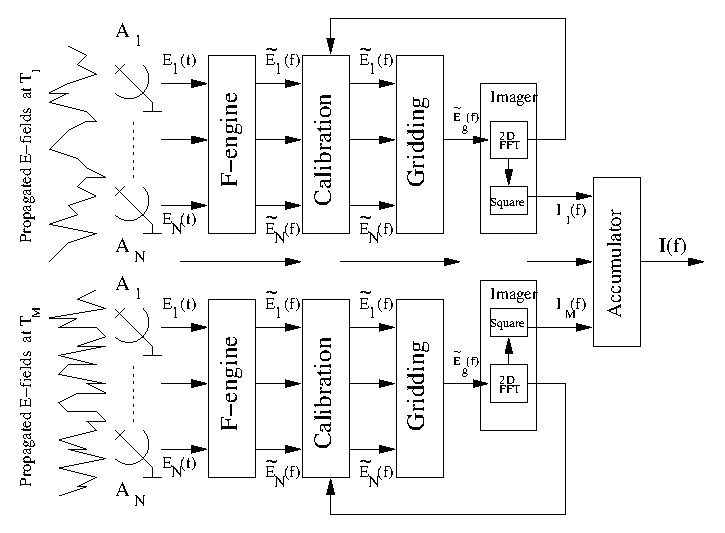
\includegraphics[width=\columnwidth]{MOFF_flowchart.eps}
  \caption{A flowchart of MOFF imaging in EPIC. The propagated electric fields
    shown on the left are measured as time-series $E_1(t)\ldots E_\textrm{N}(t)$
    by the antennas which are then Fourier transformed by the F-engine to produce
    electric field spectra $E_1(f)\ldots E_\textrm{N}(f)$. They are calibrated and
    gridded. The gridded electric fields $E_\textrm{g}(f)$ from each time series
    are imaged to produce an images $I_1(f)\ldots I_\textrm{N}(f)$. These images
    are time-averaged to obtain the final image $I(f)$.}
  \label{fig:MOFF-flowchart}
\end{figure}

Fig.~\ref{fig:FX-flowchart} shows the flowchart for software holographic
imaging from a FX correlator. The antenna-based F-engine is identical to that in
the MOFF processing. The electric field spectra from each antenna are then cross-
multiplied in the X-engine with those from all other antennas to obtain the
visibilities $V_\textrm{ij}(f)$ ($\mathbf{m}(\mathbf{v})$ in matrix notation).
They are calibrated and time-averaged to obtain $\langle V_\textrm{ij}(f)\rangle$
which are then gridded and imaged to obtain the image $I(f)$. The $I(f)$ obtained
from both techniques are identical as explained in \S\ref{sec:math}.
\begin{figure}
  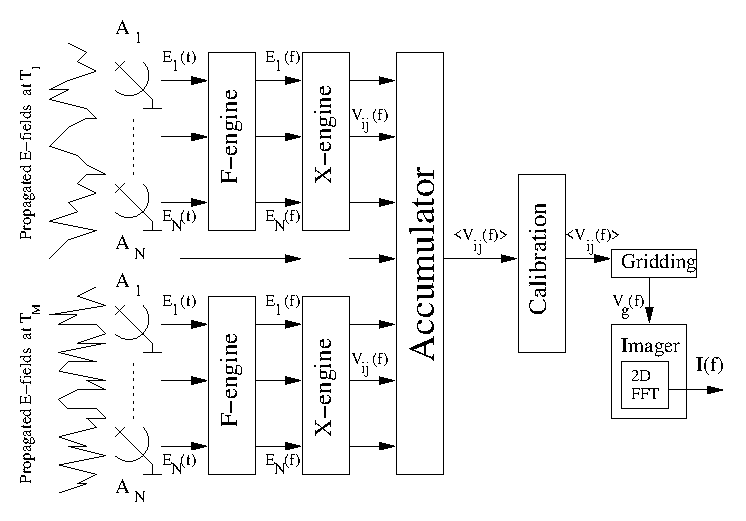
\includegraphics[width=\columnwidth]{FX_flowchart.eps}
  \caption{A flowchart of FX imaging in EPIC. The FX process flow shares the
    F-engine with the MOFF process. Following the F-engine, the electric fields
    pass through the X-engine to obtain visibilities $V_\textrm{ij}(f)$ which are
    calibrated and time-averaged. Then they are gridded to obtain the gridded
    visibilities $V_\textrm{g}(f)$ which are then imaged to obtain the image
    $I(f)$.}
  \label{fig:FX-flowchart}
\end{figure}

Here we discuss the components of these architectures in detail. 

\par\medskip
\noindent {\bf Temporal Fourier transform}
\par\medskip
\noindent This module is common to the MOFF and FX imaging techniques. Time 
samples of electric fields measured by the antenna and digitized by the A/D 
converter is Fourier transformed to generate electric field spectra. This step 
can be parallelized by antennas as shown in Fig.~\ref{fig:f-engine}. The output 
is then fed to either MOFF and FX imaging pipelines.

\begin{figure}
  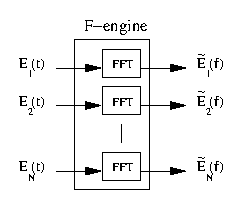
\includegraphics[width=\columnwidth]{F-engine.eps}
  \caption{Block diagram of a F-engine. The electric field data streams from
    antennas are Fourier transformed in parallel to generate electric field
    spectra.}
  \label{fig:f-engine}
\end{figure}

\par\medskip
\noindent {\bf Antenna-to-Grid Mapping}
\par\medskip
\noindent A grid is generated on the coordinate system in which antenna 
locations are specified with a grid spacing. The grid spacing can be controlled 
by the user. By default, it is set to be at $\lambda_\textrm{min}/2$ even at the 
highest frequency to ensure there is no aliasing even from regions of the sky 
far away from the field of view. The number of locations on the grid is 
restricted to be a power of 2. 

The gridding kernel in the simplest case is given by the antenna aperture
illumination function, $\widetilde{B}(\mathbf{r}-\mathbf{r}_a)$, which can
be specified either by a functional form or as a table of values against 
locations around the antennas. A nearest neighbor mapping from all antenna 
footprints to grid locations is created using an efficient k-d tree algorithm 
\citep{man99}. There is no restriction here that the aperture illumination 
function has to be identical across antennas. 

In the most general case, this gridding kernel could contain information on the
$w$-projection effect, and even other time-dependent ionospheric effects. For a
stationary antenna array in the absence of any time-dependent effects, this
mapping must only be determined once in the antenna array coordinate frame. The
antenna-to-grid mapping matrix, $\mathbf{M}(\mathbf{r},\mathbf{a})$ is described
as a transformation matrix from the space of measured electric fields by the 
antennas ($\mathbf{a}$) to the antenna array grid denoted by the coordinate 
$\mathbf{r}$. Since each antenna occupies a footprint typically the size of its 
aperture, $\mathbf{M}(\mathbf{r},\mathbf{a})$, which is generally of size
$N_\textrm{grid}\times N_\textrm{a}$, reduces to a sparse block-diagonal matrix
with only $N_\textrm{a}$ blocks and roughly $N_\textrm{k}$ non-zero entries per
block. This sparse matrix is stored in a Compressed Sparse Row (CSR) format. 
Fig.~\ref{fig:a2g-mapping} illustrates the antenna-to-grid mapping
matrix and the grid containing the mapped aperture footprints of the antennas.

\begin{figure}
  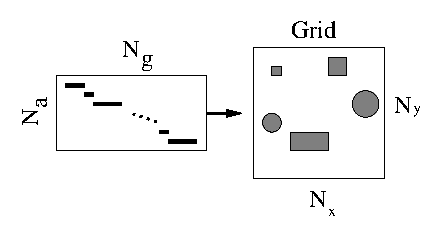
\includegraphics[width=\columnwidth]{a2g_mapping.eps}
  \caption{Block diagram of an antenna-to-grid mapping. A sparse block-diagonal
    matrix of total size $N_\textrm{grid}\times N_\textrm{a}$ is created where each
    block contains roughly the number of pixels covered by the respective kernel.
    The antenna aperture illumination kernels do not have to be identical to each
    other. A discrete set of arbitrarily placed antennas are now placed onto a
    regular grid.}
  \label{fig:a2g-mapping}
\end{figure}

\par\medskip
\noindent {\bf Calibration}
\par\medskip
\noindent Calibration of direct imaging correlators remains a challenge. Contrary
to the FX data flow, direct imagers mix the signals from all antennas before
averaging and writing to disk. It is therefore essential to apply gain solutions 
before the gridding step. Previous efforts have resorted to applying FX-generated
calibration solutions \citep{zhe14,fos14}, or integrating a dedicated FX 
correlator which periodically forms the full visibility matrix 
\citep{wij09,dev09}. 

In a companion paper to appear soon, we demonstrate a novel calibration 
technique (EPICal) which leverages the data products formed by direct imaging 
correlators to estimate antenna complex gains. This method correlates the antenna 
electric field signals with an image pixel form the output of the correlator in 
the feedback calibration fashion outlined in \citealt{mor11} (illustrated in Fig. 
\ref{fig:MOFF-flowchart} by the arrow leading from the imager to the calibration 
block). Furthermore it allows for arbitrarily complex sky models, and following 
the MOFF algorithm places no restriction on array layout, and accounts for 
non-identical antenna beam patterns. Because only a single correlation is needed 
for each antenna, the computation complexity scales only as $N_{\mathrm{ant}}$. 

The calibration module included in the EPIC repository allows for application of 
pre-determined calibration solutions, or can solve for the complex gains using 
the EPICal algorithm.

\par\medskip
\noindent {\bf Gridding Convolution}
\par\medskip
\noindent The antenna array aperture illumination over the entire grid,
$\widetilde{\mathbf{W}}(\mathbf{r})$, is obtained by a projection of the 
individual antenna aperture illuminations:
\begin{align}\label{eqn:gridding-convolution}
  \widetilde{\mathbf{W}}(\mathbf{r}) &= \sum_a \widetilde{\mathbf{W}}_a(\mathbf{r}-\mathbf{r}_a) \\
                            &= \mathbf{M}(\mathbf{r},\mathbf{a})\,\mathcal{I}(\mathbf{a}),
\end{align}
where, $\mathcal{I}(\mathbf{a})$ is a row of ones. This is achieved by
efficient multiplication with the sparse matrix created in the antenna-to-grid
mapping process using the sparse matrices module in Python's SciPy package. 
Unless $\widetilde{\mathbf{W}}(\mathbf{r})$ includes time-dependent
effects of the ionosphere or the instrument, it needs to be computed just once
for the entire observation. However, the gridding of electric fields must be
computed at every readout of the electric field spectra,
\begin{align}
  \widetilde{\mathbf{E}}(\mathbf{r}) &= \mathbf{M}(\mathbf{r},\mathbf{a})\,\widetilde{\mathbf{E}}(\mathbf{a}).
\end{align}
% The sentence below was already stated earlier.
%In practice the grid is set to be a power of 2 such that the grid spacing is at
%most $\lambda/2$ even at the highest frequency in the observing band. 

\par\medskip
\noindent {\bf Spatial Fourier Transform}
\par\medskip
\noindent Before the spatial Fourier transform, the gridded electric fields are 
padded with zeros in order to match the grid size and angular size of each image 
pixel that would have been obtained with software holography of output from an FX
correlator. 

In MOFF imaging, these are spatially Fourier transformed followed by a squaring
operation at every timestamp for every frequency channel. In FX imaging, the
spatial Fourier transform is performed only once per integration timescale and
does not include a squaring operation.

\par\medskip
\noindent {\bf Time-averaging}
\par\medskip
\noindent In MOFF imaging, the measured antenna electric fields and the 
corresponding holographic electric field images are zero-mean stochastic 
quantities. Hence, they cannot be time-averaged to reduce noise. The statistical 
quantity stable with time in this case are the square of the holographic 
electric field images. Thus, squared images have to be formed at every instant 
of time before averaging as indicated in equation~\ref{eqn:dirty-image-MOFF}.

In contrast, visibilities measured by an antenna are statistically stable within
an integration time interval. Hence, they are averaged after calibration as shown
in equation~\ref{eqn:cc-vis}. It is advantageous to average them in visibilities
before imaging because the repeated cost of spatial FFT can be avoided. Since 
this averaging has been performed already on the visibilities over an integration 
timescale, the imaging step has to be performed only once per integration cycle. 
% FX imaging holds this advantage as long as the square of the number of antennas 
% is smaller than the number of pixels on the image. 

\subsection{Software Architecture}\label{sec:software-modules}

EPIC is built using object oriented programming in Python and is built on
carefully crafted modules which closely represent real-life entities in radio 
interferometer arrays and observations. The essential modules along with their
key attributes and methods are illustrated in Fig.~\ref{fig:software-modules}.
These modules are described below.

\begin{figure*}
  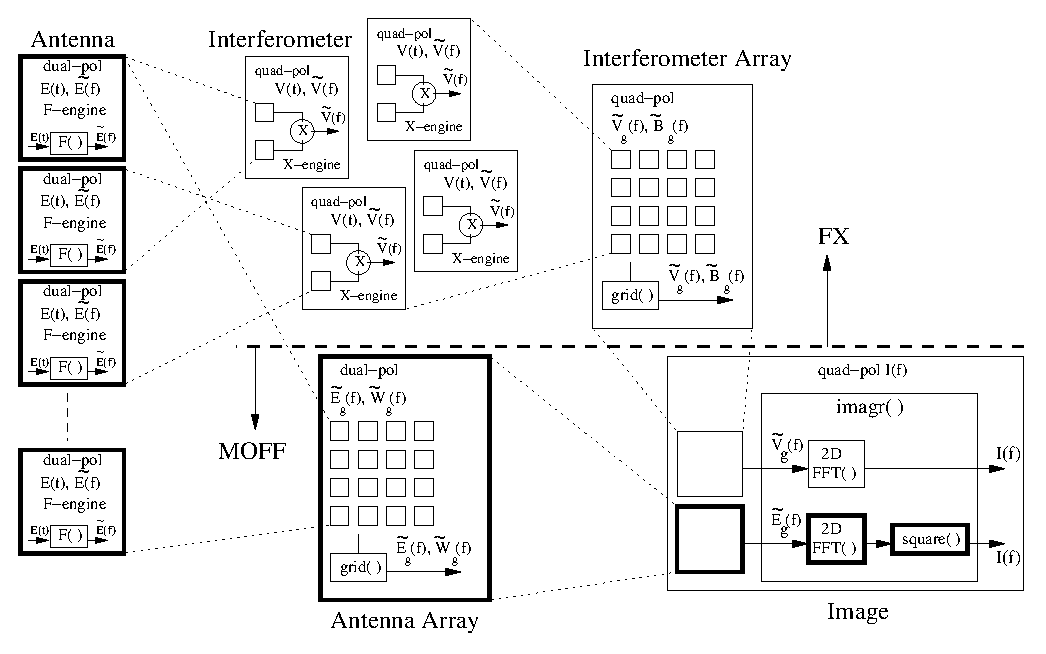
\includegraphics[width=\linewidth]{EPIC-modules.eps}
  \caption{Software architecture of EPIC with core modules, their essential
    attributes and functions. The Antenna module forms the fundamental building 
    block. It consists of electric field time-series and spectra and the 
    F-engine that performs a temporal FFT to obtain electric field spectra from 
    the time-series. The Interferometer module is made of a pair of Antenna 
    modules. Its main function is the X-engine (FX or XF) to produce visibility 
    spectra. The Antenna Array module is made of all individual Antenna modules
    as its components and contains collective properties about the antenna 
    subsystems. Its core function is the creation of antenna-to-grid mapping and 
    that of gridded aperture weights and electric fields. The Interferometer 
    Array module is very similar in principle to the Antenna Array module 
    except it operates on cross-correlations and produces gridded visibilities.
    The Image module takes gridded electric fields or visibilities and performs
    a two-dimensional spatial FFT (and squares the intermediate image in case 
    of the former) to produce output images.}
  \label{fig:software-modules}
\end{figure*}

\subsubsection{Antenna module}

The Antenna module is a fundamental building block upon which all the other 
modules are built. There is one Antenna module per antenna each having 
attributes -- the propagated electric field time-series, $E(t)$, and spectrum 
$E(f)$ for both polarizations. The most important function inside this module 
is the F-engine that Fourier transforms time-series electric field data into 
spectrum. 

The other function (not shown in the figure) is to update the data as new data 
keeps streaming in. This can also be parallelized. Another important attribute
(not shown in figure) are antenna flags for each polarization appropriate for 
the data stream being held by the Antenna module. 

\subsubsection{Interferometer module}

The Interferometer module holds the attributes and functions pertaining to
a pair of antennas and represents the cross-correlation information obtained
from the pair. Its important attributes are the two Antenna modules. It also
contains four cross-polarized visibility time-series and spectra. 

The most important function of the Interferometer module is the X-engine. 
This is essentially a software analog of hardware correlators of real 
telescope systems. The X-engine can be toggled between two states of operation,
namely, the FX and XF modes. The FX mode obtains the electric field spectra, 
$E(f)$ from the individual Antenna modules inside the Interferometer module and
multiplies the two to obtain visibility spectra, $V(f)$. On the other hand, the
XF mode cross-correlates the electric field time-series from its Antenna modules
to obtain the visibilities as a function of lags, $V_t(t)$, which is then Fourier 
transformed to obtain $V(f)$. Both modules can operate on dual-polarizations to
obtain all four cross-polarizations.

The other attributes (not shown in figure) are the flags applicable for each
cross-polarization for the current data stream. Similar to the Antenna module,
it has an update function that can update the visibilities $V_t(t)$ or $V(f)$
directly rather than through the electric fields of its component antennas. 
This functionality is to allow EPIC to operate while attached to the backend 
of traditional correlator systems. Currently, this feature is not utilized 
for purposes of this paper.

The Interferometer module forms the fundamental unit for the InterferometerArray
module (to be discussed below) and in general for visibility based correlator 
and imaging systems. 

\subsubsection{Antenna Array module}

The AntennaArray module consists of all the Antenna modules as its attributes
and represents the collective properties of its component antennas. By virtue of 
holding each antenna data independently in their respective modules the F-engine 
for the entire array can be distributed to the F-engines of the component 
antenna modules thus achieving a highly parallelized F-engine while emulating 
real telescope systems.

The most important attributes held by this module are the antenna aperture 
illumination weights and electric fields projected on the grid using the 
gridding convolution method described above and implemented by the gridding 
function (denoted by grid()) in this module. Significant parts of the 
antenna-to-grid mapping and gridding convolution are parallelizable 
across antennas and frequencies.

Individual antenna flags are carried over as additional weights to be applied
to the gridded aperture illumination and electric fields. A series of data 
streams can be stacked up to take advantage of the array optimization available 
in Python. This module is also equipped to manage dual-polarization. 

\subsubsection{Interferometer Array module}

Similar to the AntennaArray module, the InterferometerArray module consists of
individual Interferometer modules. It can parallelize the correlator operations
by distributing the X-operation over the X-engines of its component 
Interferometer modules. The interferometer-to-grid mapping and gridding 
convolution are very similar in nature to that of the Antenna Array module. 
Flag-based grid weights, stacking and ability to handle all four 
cross-polarizations are built into this module. 

\subsubsection{Image module}

The Image module is built as a general purpose module that can switch between 
operating on gridded electric fields or visibilities. At its heart, it consists
of a two-dimensional FFT where the padding can be specified by the user to 
control the resolution in the output images. In case of electric field based
imaging, there is an additional step of squaring the holographic electric field
images. This is packaged into the function annotated as imagr().

Besides its core functions of spatial Fourier transform and squaring, it can 
stack, accumulate and average images, and optionally remove the antenna
auto-correlations centered around the zero-spacing pixel in the $uv$ plane. 
It also handles all four cross-polarization products. Currently, it can 
support writing data out in standard FITS format. 

\section{Verification}\label{sec:verify}

In order to prove the accuracy of the EPIC code, we verify the images produced 
through simulations. We simulate electric field streams from a model sky and 
process the data through both the MOFF and visibility based imaging algorithms. 
We then compare the output images to demonstrate their equivalence.

\subsection{Dealing with antenna auto-correlations}\label{sec:rm-autocorr}

Before diving into the details of simulations and comparison with visibility 
based imaging, we describe the elimination of a minor mathematical difference 
between the two techniques. The squaring operation under MOFF imaging in the 
image plane introduces antenna auto-correlations around the zero spacing in 
the $uv$-plane which are absent in traditional visibility-based imaging. In 
order to facilitate a robust comparison, these auto-correlations are removed 
from both the $uv$ and image planes, which is otherwise not an essential part 
of the core algorithm. We describe below how they can be removed from the $uv$ 
plane in a straightforward manner. 

The shape and extent of these auto-correlations can be estimated from the 
antenna aperture illumination pattern. The aperture illumination patterns
are already available from the gridding step. Fig.~\ref{fig:autocorr_wts_PB} 
shows the estimated weights from antenna auto-correlations in the $uv$-plane 
(left) and the corresponding response in the image plane (right). The latter 
is simply the directional antenna power response. 

\begin{figure}
  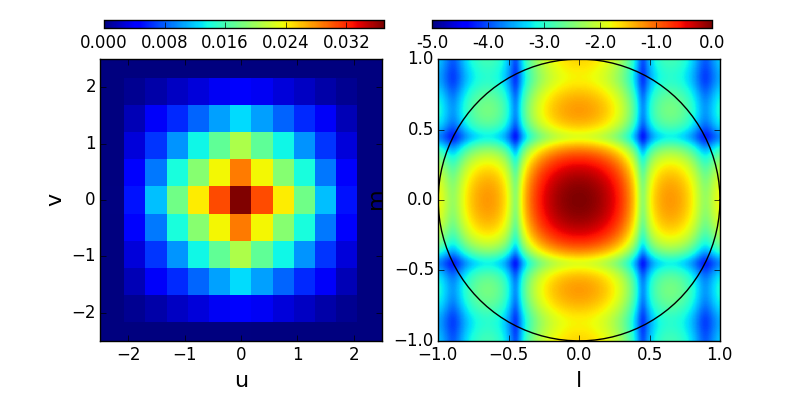
\includegraphics[width=\columnwidth]{autocorr_uvwts_pbeam.png}
  \caption{The auto-correlation of weights of a square shaped antenna aperture
    in the $uv$ plane (left) and the corresponding directional antenna power 
    response on the sky (right) in coordinates specified by direction cosines. 
    The antenna auto-correlation weights are normalized to a sum
    of unity yielding a peak response of unity in the antenna's directional
    power pattern on the sky. The color scale for the directional power 
    pattern is logarithmic. The black circle indicates the sky horizon and
    values beyond it are not physical and hence ignored.}
  \label{fig:autocorr_wts_PB}
\end{figure}

We inverse Fourier transform the squared images and beams back to the $uv$ 
plane and subtract the estimated auto-correlation kernel scaled to the peak 
value centered at the zero spacing pixel. The final averaged image is obtained 
by Fourier transforming the $uv$ plane data and weights with the 
auto-correlations subtracted to the image plane. These images are now comparable 
to those obtained from visibility-based imaging. This step of removing 
auto-correlations is optional and required to be performed only once per 
integration timescale and does not add significant cost to the full operation.

\subsection{Simulations}\label{sec:sim}

We use the EPIC simulator to generate electric field samples from a sky model. In
our simulations, we use 64 frequency channels each of width $\delta f = 40$~kHz, 
10 point sources of flux densities 10~Jy at random locations. The number of
timestamps integrated in one integration cycle was kept at eight where each A/D 
timeseries is $1/\delta f=25\,\mu$s long. We use the MWA array layout 
\citep{bea12} for demonstration. Only the inner 51 tiles within a square bounding
box of 150~m on each side were used. We assumed all tiles are identical and have 
a square shaped electric field illumination footprint 4.4~m on each side. 

Fig.~\ref{fig:MOFF-FX-image} shows the dirty images (top) and synthesized beams
(bottom) obtained with antenna-based MOFF and FX visibility-based imaging 
algorithms packaged in EPIC. The antenna auto-correlations that correspond to 
zero spacing have been removed from the MOFF image and the corresponding 
synthesized beam. The sky positions of the simulated sources are indicated by 
solid black circles. The reconstructed sky image has the simulated sources at the
expected sky positions in either case. Both algorithms result in images and 
synthesized beams that are well matched with each other. Their fluxes are 
modulated by a multiplicative power pattern corresponding to that of a uniform
square aperture. 

\begin{figure}
  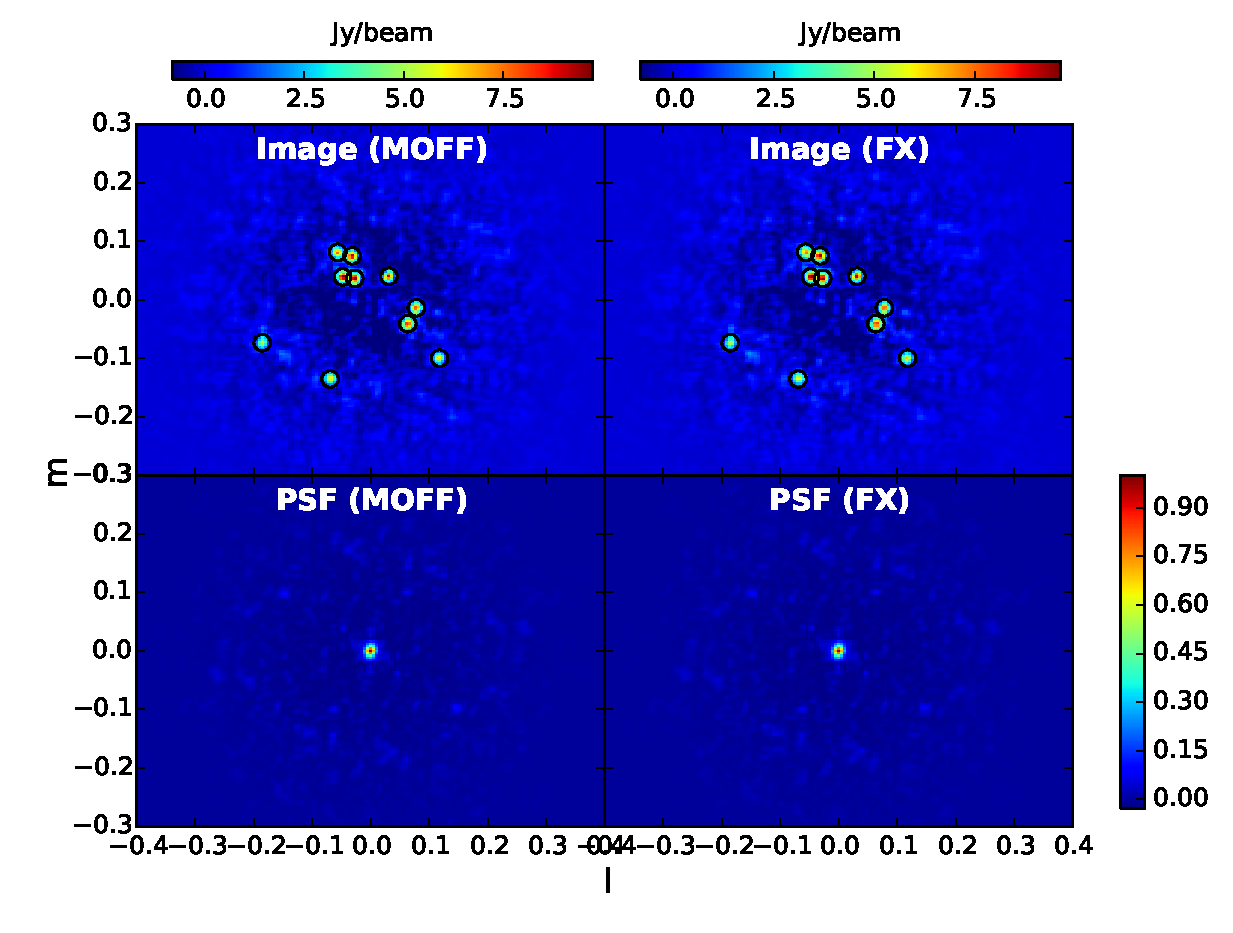
\includegraphics[width=\columnwidth]{MOFF_FX_image_comparison.eps}
  \caption{Dirty images (top) and synthesized beams (bottom) obtained from 
    simulated data using antenna-based MOFF algorithm (left) and FX 
    visibility-based software holography (right). The solid black circles in the
    top panels indicate the simulated source positions. The antenna 
    auto-correlations at zero-spacing have been removed from the MOFF images. 
    The images in either case reconstruct the sources at the right locations 
    with the fluxes expected after multiplication by the antenna power pattern. 
    The synthesized beams from the two algorithms are well matches in size and
    shape. The overall modulation by the power pattern is seen clearly in both
    images.}
  \label{fig:MOFF-FX-image}
\end{figure}

\subsection{Comparison of outputs}\label{sec:diff}

We investigate the two imaging algorithms for differences from the point of 
view of the quality of their outputs. We begin by comparing the gridded 
cross-correlation weights in the $uv$-plane. In MOFF imaging, weights 
from antenna auto-correlations have been removed as described in 
\S\ref{sec:rm-autocorr}. 

Fig.~\ref{fig:MOFF-FX-uvwts} shows the cross-correlation weights obtained 
with MOFF imaging (left) and visibility-based imaging (right). The first 
notable difference is in the weights around zero spacing. Though both show a
dominant void around zero-spacing, the void obtained with MOFF algorithm shows 
many pixels with non-zero weights. In contrast, the zero-spacing void from 
traditional imaging consists of predominantly zero-valued pixels. The gridding
process in the former involves rounding the antenna footprint to the nearest 
grid pixel. Depending on the exact location of the center of the antenna 
relative to the grid, the grid pixels that receive contribution from an
antenna may be a pixel narrower along one or both axes relative to that from
another identical antenna but with a different center location relative to the
grid. The resulting auto-correlation footprint will also not necessarily be 
identical. Hence, using a single expected footprint for subtraction will
typically leave some residuals behind as seen in the void region in the 
weights obtained with MOFF imaging. 

These residuals can be mitigated by: 
\begin{enumerate}
  \item making the grid spacing finer which makes the rounding error less 
    susceptible to the location of the antenna center relative to the grid, 
    and
  \item subtracting each auto-correlation of antenna weights separately by 
    using the shape and extent of the footprint appropriate for that specific
    antenna aperture. 
\end{enumerate}
The latter is the most general solution applicable especially in the case of 
heterogeneous antenna arrays and is under active development for EPIC.

The other notable difference is that weights outside the zero-spacing void in
some regions are different from each other at the few percent level though the 
sum of weights in these regions are identical. For instance, note the 
difference in weights at $(u,v)\approx (2,-10)$. This is found to arise 
because with MOFF imaging the antenna locations were rounded to the nearest 
grid pixel whereas in visibility-based imaging the baseline locations 
(difference between antenna locations) were rounded to the nearest grid pixel. 
Since rounding is not a commutative operation (i.e. rounding of the difference 
value is not necessarily equal to the difference of the rounded values), the 
gridding operation in the two cases introduces rounding errors in the placement 
of antenna aperture and cross-correlated aperture weights. Each antenna 
aperture weight projected to the nearest grid location can be displaced by 
$\sim 1$--2 pixels. This effect can be mitigated only by making the grid 
spacing finer at the expense of increased computational cost. 

\begin{figure}
  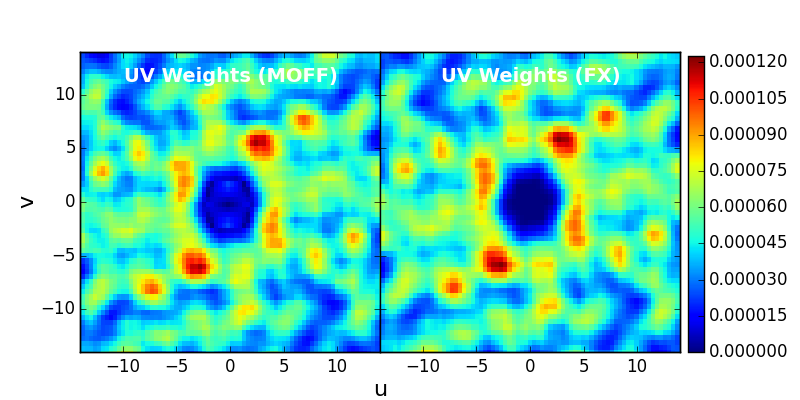
\includegraphics[width=\columnwidth]{MOFF_FX_comparison_uvwts_test_aperture_zero_spacing_removed.png}
  \caption{Dirty images (top) and synthesized beams (bottom) obtained from 
    simulated data using antenna-based MOFF algorithm (left) and FX 
    visibility-based software holography (right). The solid black circles in the
    top panels indicate the simulated source positions. The antenna 
    auto-correlations at zero-spacing have been removed from the MOFF images. 
    The images in either case reconstruct the sources at the right locations 
    with the fluxes expected after multiplication by the antenna power pattern. 
    The synthesized beams from the two algorithms are well matched in size and
    shape. The overall modulation by the power pattern is seen clearly in both
    images.}
  \label{fig:MOFF-FX-uvwts}
\end{figure}

% The synthesized beam can be written as:
% \begin{align}\label{eqn:syn-beam}
%   B(\hat{\mathbf{s}}) &= \left| \sum_\mathbf{r} \widetilde{W}(\mathbf{r})\,e^{-i2\pi\mathbf{r}\cdot\hat{\mathbf{s}}}\right|^2, \\
%   \textrm{or}, \quad B(l,m) &= \left| \sum_{r_x,r_y} \widetilde{W}(r_x,r_y)\,e^{-i2\pi(r_x l + r_y m)}\right|^2 
% \end{align}
% where, $\hat{\mathbf{s}}\equiv (l,m)$, $\mathbf{r}\equiv (r_x,r_y)$ and 
% $\widetilde{W}(\mathbf{r})$ is given by equation~\ref{eqn:gridding-convolution}.
% If the errors in the determination of $r_x$ and $r_y$ are denoted by 
% $\delta r_x$ and $\delta r_y$ respectively, the error on $B(l,m)$ can be 
% estimated using a simple propagation of errors, where,
% \begin{align}
%   \frac{\partial{B}(l,m)}{\partial{r_x}} &= e^{-i2\pi\mathbf{r}\cdot\hat{\mathbf{s}}}\left[\frac{\partial{\widetilde{W}(r_x,r_y)}}{\partial{r_x}} - i 2\pi l\widetilde{W}(\mathbf{r})\right] \label{eqn:syn-beam-pdev1}\\
%   &\qquad\qquad \times \sum_{\mathbf{r}^\prime} \widetilde{W}^\star(\mathbf{r}^\prime)\,e^{+i2\pi\mathbf{r}^\prime\cdot \hat{\mathbf{s}}} \\
%   &= e^{-i2\pi\mathbf{r}\cdot\hat{\mathbf{s}}}\left[\frac{\partial{\widetilde{W}(r_x,r_y)}}{\partial{r_x}} - i2\pi l\widetilde{W}(\mathbf{r})\right]\,W^\star(\hat{\mathbf{s}}), \\
%   \textrm{and},\frac{\partial{B}(l,m)}{\partial{r_y}} &= e^{-i2\pi\mathbf{r}\cdot\hat{\mathbf{s}}}\left[\frac{\partial{\widetilde{W}(r_x,r_y)}}{\partial{r_x}} - i2\pi m\widetilde{W}(\mathbf{r})\right]\,W^\star(\hat{\mathbf{s}}). \label{eqn:syn-beam-pdev2}
% \end{align}
% It must be noted that although we start with a squaring operation in 
% equation~\ref{eqn:syn-beam}, in equations~\ref{eqn:syn-beam-pdev1} through 
% \ref{eqn:syn-beam-pdev2}, the summations are performed only when 
% $\mathbf{r}\ne \mathbf{r}^\prime$ and therefore do not include the 
% auto-correlations of the antenna weights. The error expected in $B(l,m)$ is:
% \begin{align}
%   \left|\delta B(l,m)\right|^2 &= \sum_{r_x}\left|\frac{\partial{B}(l,m)}{\partial{r_x}}\right|^2 \delta r_x^2 + \sum_{r_y}\left|\frac{\partial{B}(l,m)}{\partial{r_y}}\right|^2 \delta r_y^2 \\
%   &= \delta r_x^2 \sum_{r_x}\left|\frac{\partial{\widetilde{W}(r_x,r_y)}}{\partial{r_x}} - i2\pi l\widetilde{W}(\mathbf{r})\right|^2\,\left|W(\hat{\mathbf{s}})\right|^2 \nonumber\\
%   &\qquad + \delta r_y^2 \sum_{r_y}\left|\frac{\partial{\widetilde{W}(r_x,r_y)}}{\partial{r_y}} - i2\pi m\widetilde{W}(\mathbf{r})\right|^2\,\left|W(\hat{\mathbf{s}})\right|^2
% \end{align}
% For the current simulations, 
% \begin{align}
%   \delta r_x = \delta r_y &\simeq 1, \\
%   \widetilde{W}(r_x,r_y) &= \{0, \textrm{constant}\}, \\
%   \textrm{and},\qquad \frac{\partial{\widetilde{W}(r_x,r_y)}}{\partial{r_x}} &= \frac{\partial{\widetilde{W}(r_x,r_y)}}{\partial{r_y}} = 0.
% \end{align}
% Hence,
% \begin{align}
%   \left|\delta B(l,m)\right|^2 &\simeq 4\pi^2\left(l^2+m^2\right)\,B(\hat{\mathbf{s}})\,\sum_\mathbf{r}\,\left|\widetilde{W}(\mathbf{r})\right|^2, \\
% \textrm{or},\qquad \left|\delta B(l,m)\right| &\simeq 2\pi\sqrt{l^2+m^2}\,\left|W(\hat{\mathbf{s}})\right|\,\left(\sum_\mathbf{r}\,\left|\widetilde{W}(\mathbf{r})\right|^2\right)^{1/2}, \label{eqn:syn-beam-error}
% \end{align}
% where, $B(\hat{\mathbf{s}}) \equiv \left|W(\hat{\mathbf{s}})\right|^2$. Thus, 
% the error on the synthesized beam is proportional to the antenna power pattern
% and increases linearly outward in radial bins of direction cosines.

We study the effect of the differences in gridded weights on the image plane. 
Fig.~\ref{fig:psf-diff} shows the difference between the synthesized beams 
obtained with the two methods. A difference map between the two synthesized 
beams is shown on top. The amplitude of the difference appears to be 
modulated by the directional power response of the antenna. At the bottom, 
in radial bins, the rms of the synthesized beam (gray) and the rms of the 
difference map (black) are plotted in percentage units relative to the peak 
(to be read using the axis on the left side of the plot). The antenna power 
pattern (red; to be read using the scale on the right) is plotted for reference. 

\begin{figure}
  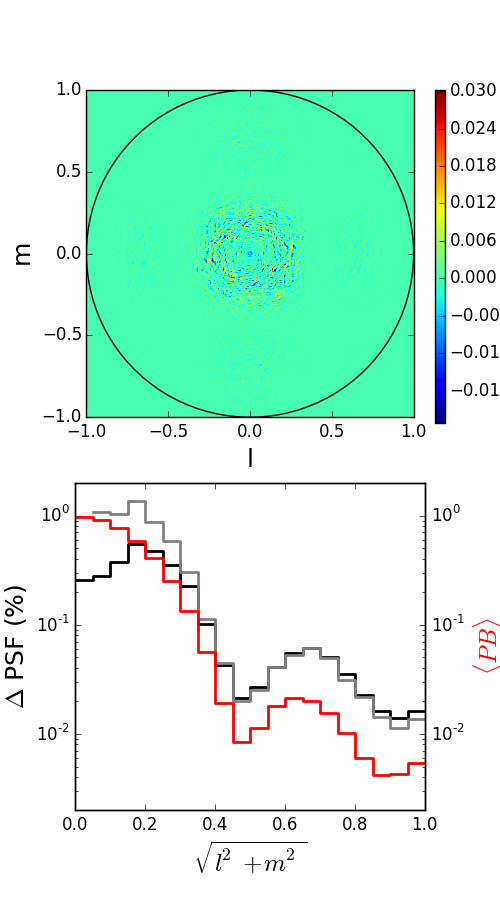
\includegraphics[width=\columnwidth]{diff_psf_MOFF-FX_test_aperture.png}
  \caption{Map of difference between the synthesized beams obtained with the 
    two methods (top) and radial statistics of the synthesized beams and 
    their differences (bottom). The maximum difference is of the order of a 
    few percent. The difference appears to be modulated in amplitude by the 
    power pattern of the antenna. }
  \label{fig:psf-diff}
\end{figure}

The synthesized beam rms is proportional to the antenna power pattern as 
expected from a point spread function uncorrected for the antenna power 
pattern. The rms of differenced synthesized beams is 
also modulated by the antenna power pattern. The rms of the difference is 
definitely lesser than the rms of the synthesized beam in the central regions 
up to $(l^2+m^2)^{1/2}\lesssim 0.3$. This implies that the beams are well 
matched in the central regions. In the outer regions, their mismatch is 
comparable to the rms of synthesized beams. This indicates the two 
synthesized beams are not completely randomly different from each other in
which case the rms of the difference would have been $\approx \sqrt{2}$
higher than the rms of the each of the synthesized beams. This indicates 
that while differences exist, large fractions of them are still well matched
to each other even out to the horizon. Thus the rounding errors in gridding 
do not affect the statistics of the images or the synthesized beams.

\subsection{Application to LWA data}\label{sec:LWA-data}

Here we demonstrate our software using narrow band data from the LWA in New 
Mexico. This data is in LWA narrow-band transient buffer (TBN) format with 512 
voltage time samples from 255 antennas within roughly a diameter of 100~m. The 
data is centered at a frequency of 74.03~MHz, with a sample rate (equal to the 
bandwidth) of 100~kHz with 512 complex time samples in a A/D writeout timescale 
of 5.12~ms, a frequency resolution of 195.3125~Hz and dual polarization. There 
are 391 such timestamps yielding a total duration of 2~s. 

We corrected the cable delays, but otherwise assume the data is sufficiently 
calibrated to image directly. A test of EPICal on this data will be conducted 
in the future.

Fig.~\ref{fig:LWA-image} shows the image produced with MOFF imaging 
packaged in EPIC after averaging over the entire 2~s of data and the inner
$\approx 80$\% of bandwidth (roughly 80~kHz). The image is shown in direction 
cosine coordinates -- $l$ along x-axis and $m$ along y-axis. The flux scale 
is arbitrary. Even in this proof-of-concept demonstration, we see Cyg~A and 
Cas~A prominently and Sgr~A faintly as annotated, thus validating the 
functionality of the EPIC package.

\begin{figure}
  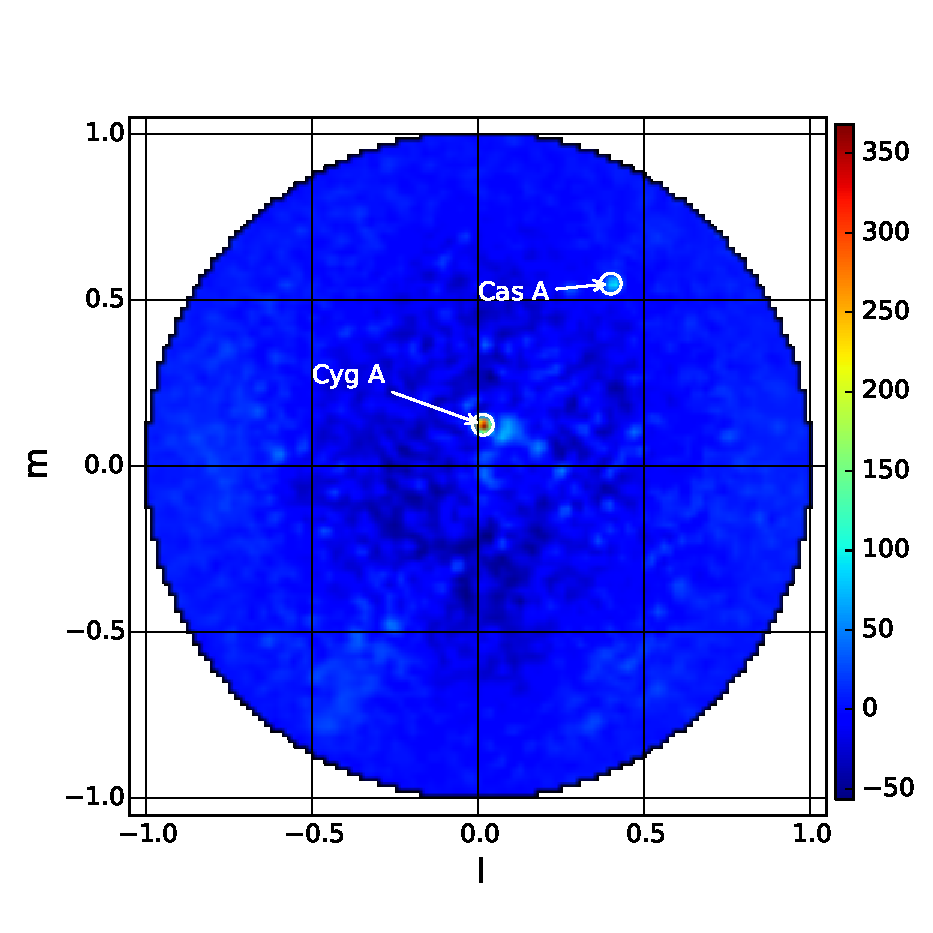
\includegraphics[width=\columnwidth]{LWA_MOFF_bandavg_image_4_iterations_analytic_aperture.eps}
  \caption{Image from LWA TBN data obtained with MOFF imaging using EPIC 
    package after averaging over 2~s and $\approx 80$~kHz. The x- and y-axes
    denote direction cosines $l$ and $m$ respectively. The antenna voltages
    are compensated for their respective delays. The flux scale is arbitrary
    and not calibrated. Locations of Cyg~A, Cas~A, Sgr~A, Her~A and Jupiter
    are annotated.}
  \label{fig:LWA-image}
\end{figure}

\section{Analysis and Feasibility}\label{sec:analysis}

We now investigate the feasibility of implementing the EPIC imager on current
and future radio telescopes. 

We have profiled the core routines of EPIC line-by-line for various ranges of 
parameters such as antenna filling fraction, maximum baseline length, bandwidth 
and frequency resolution, integration timescale, etc. for HERA antenna layouts 
which are highly compact. However, we note that in general, the hardware and 
optimization of routines in place will determine the relative speeds of the 
different stages in the pipeline. 

Of all steps in the MOFF pipeline that are repeated for every writeout from 
the F-engine, the slowest step even for dense HERA layouts is found to be the 
spatial two-dimensional FFT in the imaging stage relative to applying the sparse 
matrix gridding convolution, squaring or time-averaging. For instance, even in 
the dense array layout scenario that makes these stages perform the slowest, the 
gridding convolution, squaring and time-averaging take up only $\simeq 40$\%, 
$\simeq 40$\% and $\simeq 15$\% respectively of the time taken by the spatial 
Fourier transform. With sparser arrays the gridding process will be be even 
faster. 

In the visibility-based imaging, the predominant computational cost is at
the X-engine requiring $N_\textrm{a}(N_\textrm{a}-1)/2$ complex multiplications 
per channel at every correlator writeout timescale. 

In the following discussions, we will assume that the computational cost for
the MOFF imaging is determined by the spatial Fourier transform while  
that for visibility-based imaging comes from $N_\textrm{a}(N_\textrm{a}-1)/2$ 
cross-correlations. However, if non-linearities such as non-coplanarity of 
baselines \citep{cor08} and wide-field phenomena like the {\it pitchfork} 
effect \citep{thy15a,thy15b} are to be corrected for, the antenna based 
illumination footprint can start becoming less compact in the measurement 
plane and can result in a costlier gridding process.

The number of complex multiplications and additions in the spatial Fourier 
transform implemented via Fast Fourier Transform \citep[FFT;][]{coo65} is 
$\approx \beta N_\textrm{g}\log N_\textrm{g}$ where $N_\textrm{g}$ 
is the number of pixels on the grid and $\beta$ is a constant that depends on 
the implementation of twiddle FFT algorithms \citep{bri74}. In our study, we 
set $\beta=5$, a value much more conservative than was indicated in 
\citet{mor11}. We set the number of complex multiplications in the X-engine 
in visibility based imaging to $N_\textrm{a}^2$.

We consider a variety of current and planned radio telescopes. Their antenna 
layouts are summarized in Table~\ref{tab:antenna-layouts}. The size of the 
layout gives the maximum baseline $b_\textrm{max}$. The grid spacing is 
determined by the science goals of the experiment in general. For our 
purpose, we assume a typical requirement that only the field of view of the 
antenna is to be imaged. This sets the grid spacing to be equal to the size 
of the antenna, $A_\textrm{a}$. Hence, 
$N_\textrm{g}\simeq b_\textrm{max}^2/A_\textrm{a}$. 

\begin{table}
  \centering
  \caption{Radio telescopes and array layouts.}
  \label{tab:antenna-layouts}
  \begin{threeparttable}
  \begin{tabular}{ccccc} 
    \hline
    Telescope & Core & Number & Antenna & Frequency \\
              & size & of Antennas & size & \\
              & $b_\textrm{max}$ (in m) & $N_\textrm{a}$ & $A_\textrm{a}$ (in m$^2$) & $f_0$ (in MHz) \\
    \hline
    MWA-112\tnote{a} & 1400 & 112 & 16 & 150 \\
    MWA-240\tnote{a} & 1400 & 240 & 16 & 150 \\
    MWA-496\tnote{a} & 1400 & 496 & 16 & 150 \\
    MWA-112\tnote{a} & 1400 & 1008 & 16 & 150 \\
    LOFAR-LC\tnote{b} & 3500 & 24 & 5809 & 50 \\
    LOFAR-HC\tnote{b} & 3500 & 48 & 745 & 150 \\
    LWA1 & 100 & 256 & 10 & 50 \\
    LWA-OV\tnote{c} & 200 & 256 & 10 & 50 \\
    HERA-19 & 70 & 19 & 154 & 150 \\
    HERA-37 & 98 & 37 & 154 & 150 \\
    HERA-331 & 294 & 331 & 154 & 150 \\
    HERA-6769\tnote{d} & 1330 & 6769 & 154 & 150 \\
    SKA1-LC\tnote{e} & 1000 & 750 & 962 & 150 \\
    SKA1-LCD\tnote{f} & 1000 & 192,000 & 962 & 150 \\
    CHIME & 100 & 1280 & 8 & 600 \\
    HIRAX & 200 & 1024 & 6 & 600 \\
    \hline
  \end{tabular}
  \begin{tablenotes}
    \item[a] MWA-N denotes N tiles in the specified core diameter
    \item[b] LC and HC denotes low band and high band stations inside the 
      specified core diameter 
    \item[c] Owens Valley LWA
    \item[d] Hypothetically chosen to have a total collecting area of 
      1~km$^2$
    \item[e] This is the number of beamformed stations expected to be in the 
      core, roughly three-fourths of the total number
    \item[f] All dipoles inside the core are used as independent elements 
      without station beamforming
  \end{tablenotes}
  \end{threeparttable}
\end{table}

Fig.~\ref{fig:parameter-space-computations-instruments} shows the number of 
complex operations per frequency channel per integration timescale. Telescopes 
that fall to the left of this line indicate MOFF imaging is computationally
more efficient than visibility based imaging. All HERA layouts except possibly
HERA-19 are in a parameter space where MOFF imaging holds the advantage. The 
solid line showing future trajectory of HERA like systems will be clearly 
favoured by MOFF imaging. The gray shaded area is for a projected LWA 
expansion and is also predominantly in the region favouring MOFF imaging. 
It is bounded by the LWA1 and LWA-OV on the left and right 
respectively. The current (see Table~\ref{tab:antenna-layouts}) and
an expanded layout with a four-fold increase in number of elements over a
50\% increase in $b_\textrm{max}$ provide the bounds at the bottom and top 
respectively. Current instruments such as MWA and LOFAR lie in parameter space
favouring visibility based imaging. 

\begin{figure}
  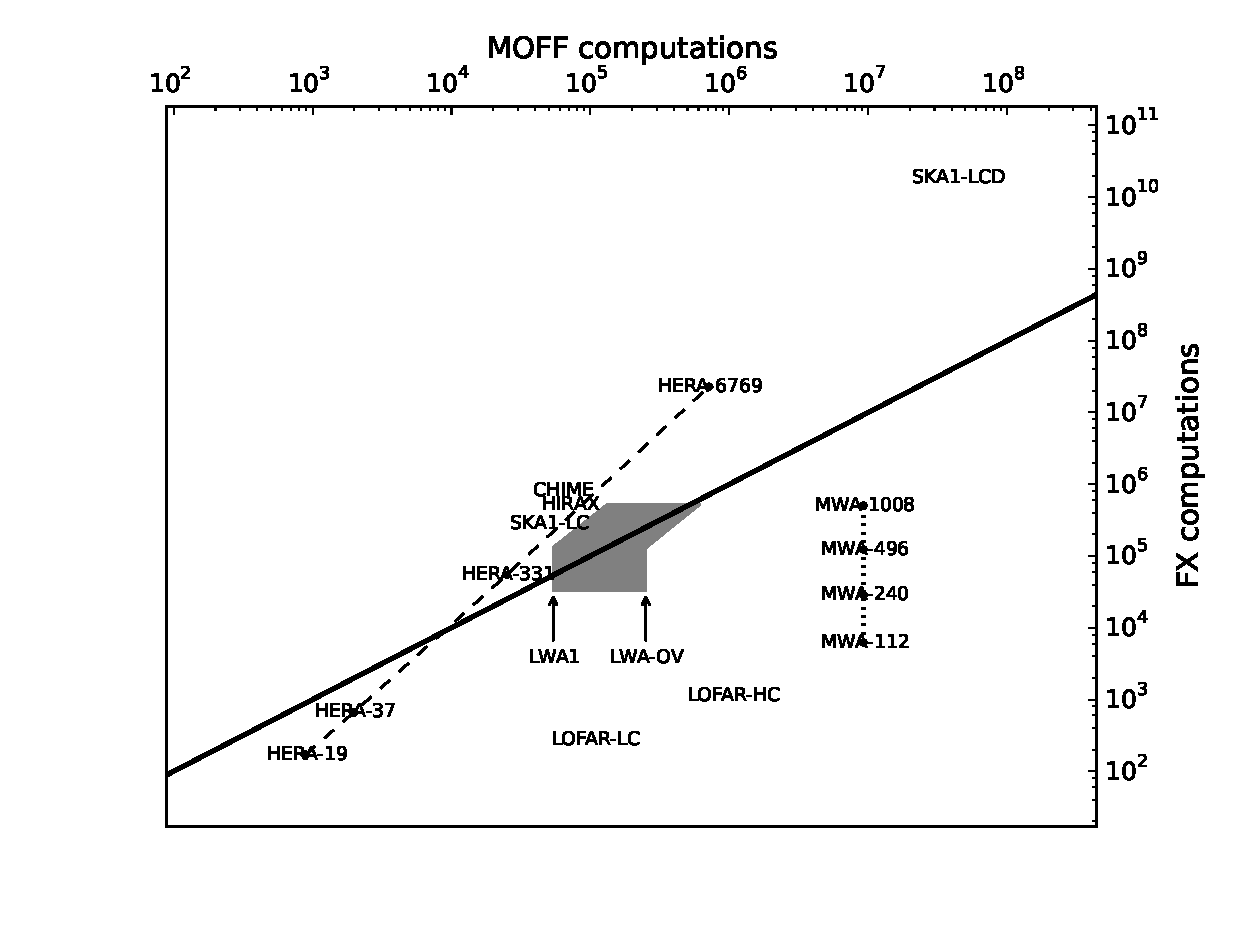
\includegraphics[width=\columnwidth]{MOFF_FX_computations_fov_gridding_annotated.eps}
  \caption{Current and planned instruments in parameter space of
    number of complex multiplies and adds with MOFF and FX. The dashed line
    is the boundary at which the number of operations with MOFF and visibility 
    based imaging are equal. MOFF imaging is more efficient for telescopes 
    occupying the left of this line and vice versa. CHIME, HIRAX and all the 
    HERA layouts except HERA-19 and HERA-37 lie in the parameter space favoured 
    by MOFF imaging. And so are SKA1-LC and SKA1-LCD. The solid black curve 
    shows the projected trajectory of bigger close-packed hexagonal layouts 
    similar to HERA. The gray shaded area denotes the projected trajectory of 
    the LWA bounded by LWA1 (left edge), LWA-OV (right edge), current layout 
    (bottom) and a four-fold increase in the number of elements within a 50\% 
    increase in the core size (top). Current instruments such as MWA and LOFAR 
    fall in a region favoured by visibility based imaging.}
  \label{fig:parameter-space-computations-instruments}
\end{figure}

We now consider antenna array layouts described by three quantities essential
to radio interferometry, namely, maximum baseline length, number of antennas,
and the size of each antenna. 

Fig.~\ref{fig:parameter-space-bll-nant-instruments} shows the ratio of the
number of computations required with visibility based imaging relative to 
MOFF imaging and the boundaries where this ratio is unity. The color scale 
refers to the ratio while using a 1~m antenna element. Pairs of black and
white lines of the same line style correspond to a specific antenna size. For 
a given antenna size (annotated on the plot), the white line denotes the 
minimum baseline length that could achieve the closest packing as a function 
of the number of antennas. Regions to the right of the white line for a 
given antenna size imply a physically impossible scenario where antennas will 
have to be packed overlapping with each other. For the same antenna size, the 
black line denotes the boundary where the ratio of the number of computations 
with either algorithm becomes unity. Regions to the right of the black lines 
favour usage of the MOFF algorithm. Thus the wedge between the white and black 
lines denotes the region in parameter space where MOFF algorithm holds a 
definite advantage while visibility based algorithms will be favoured to the 
left of the black lines. As antenna size increases the maximum number of 
antennas for a dense packing as a function of baseline length decreases. Hence 
the white lines shift leftward as antenna size increases. Similarly, with 
increase in antenna size, $N_\textrm{g}$ also decreases when field of view 
imaging is achieved with an increasing grid spacing equal to antenna size and
hence lowers the amount of computations required with the MOFF algorithm. This
shifts the black curves leftward. HERA-331, HERA-1027, LWA1, SKA1-LC and 
SKA1-LCD are inside their respective wedges indicating they are in regions that
favour the usage of MOFF imaging. For fixed baseline length, regions favouring
the MOFF algorithm tend to be towards large $N_\textrm{a}$ indicating large-N
dense array layouts with smaller antenna elements are best suited for deploying 
EPIC.

\begin{figure}
  \includegraphics[width=\columnwidth]{MOFF_FX_crossover_baseline_n-antennas_rho_fov_gridding.eps}
  \caption{Current and instruments planned for future in parameter space of
    baseline length and number of antennas with MOFF and FX. Color scale shown 
    is for the ratio of number of computations required by visibility based
    imaging to that by the MOFF algorithm. Different line styles denote 
    different antenna sizes annotated. For a given antenna size, the 
    corresponding white line denotes the maximum number of antennas that can 
    be packed inside various baseline lengths. The region to the right of the 
    white lines for corresponding antenna size is physically disallowed. 
    Regions to the left of the black lines of the same corresponding antenna 
    size (or line style) favours usage of visibility based imaging. Region 
    inside the wedge enclosed by the black and white lines favours using the 
    MOFF algorithm for any given antenna size. These wedges shift leftward with 
    increasing antenna size. HERA-331, HERA-1027, LWA1, SKA1-LC and SKA1-LCD
    are inside their corresponding wedges that favour the usage of MOFF 
    imaging.}
  \label{fig:parameter-space-bll-nant-instruments}
\end{figure}

\section{Conclusions}\label{sec:conclusions}

As radio astronomy is entering a new era, advances in instrumentation have to
be accompanied by equal advances in processing techniques to manage 
computational resources. Many future radio telescopes such as the SKA, HERA and 
LWA are headed towards the large-N dense array layout model for which 
computational cost from traditional FX/XF correlator based architecture and 
visibility based imaging starts rising steeply. We have provided the first 
software demonstration of a general purpose imaging algorithm using our generic 
and efficient EPIC software that is designed to bring this cost down from 
$\mathcal{O}(N^2)$ to $\mathcal{O}(N\log N)$. Under the class of direct imaging 
techniques, ours is one of the most generic -- neither does it place any 
constraint on the array layout to be on a regular grid nor does it require the
antenna array to be homogeneous. 

Our package, now publicly available, written in object oriented Python is 
highly modularized and parallelizable. It includes an implementation of the 
MOFF algorithm in addition to visibility based software holography imaging and 
a data simulator for sky models. It has been successfully tested on simulated 
as well as real LWA observations. 

The MOFF algorithm packaged with EPIC is already found to be most suitable 
for many present and planned radio telescopes such as the LWA, HERA and SKA. 
In general, MOFF is most suited to operate in the region of parameter space
characterized by dense packing of a large number of antennas especially when 
consisting of a large number of small antenna elements. 

A unique and significant advantage is the instantaneous availability of 
calibrated time-domain images bundled together with the hardware frontend 
such as the F-engine as an integrated module. Hence, it is a compelling 
candidate for time-domain radio astronomy, e.g. search for and monitoring of 
transients. Transient detection pipeline at the backend of EPIC can be 
fine-tuned to target fast transients such as the Fast Radio Bursts 
\citep[FRB;][]{tho13} on millisecond timescales at GHz frequencies or slow 
transients from planetary and exoplanetary origins at frequencies around 
100~MHz. 

Thus, EPIC with the MOFF algorithm packaged is uniquely poised to offer a
substantial advantage to imaging with large-N dense arrays typical of 
next-generation radio telescopes as well as push the frontiers of 
time-domain astronomy to fill gaps in understanding the science behind 
phenomena responsible for extreme transient events in the Universe.

In the near future, we plan to upgrade our current Python implementation 
of EPIC to a GPU based pipeline in order to operate on real-time data and 
develop a transient trigger and monitor backend. In the meanwhile, we plan 
to demonstrate the capability of EPIC to calibrate and image from heterogeneous 
arrays and incorporate corrections for non-coplanarity of baselines and 
direction-dependence of calibration. 

\section*{Acknowledgements}

We thank Greg Taylor for providing us the LWA data, and Larry D'Addario, 
Gregg Hallinan and Harish Vedantham for their valuable inputs. Construction of 
the LWA has been supported by the Office of Naval Research under Contract 
N00014-07-C-0147. Support for operations and continuing development of the LWA1 
is provided by the National Science Foundation under grant AST-1139974 of the 
University Radio Observatory program.

%%%%%%%%%%%%%%%%%%%%%%%%%%%%%%%%%%%%%%%%%%%%%%%%%%

%%%%%%%%%%%%%%%%%%%% REFERENCES %%%%%%%%%%%%%%%%%%

% The best way to enter references is to use BibTeX:

\bibliographystyle{../mnras}
\bibliography{../epic} % if your bibtex file is called example.bib


% Alternatively you could enter them by hand, like this:
% This method is tedious and prone to error if you have lots of references
% \begin{thebibliography}{99}
% \bibitem[\protect\citeauthoryear{Author}{2012}]{Author2012}
% Author A.~N., 2013, Journal of Improbable Astronomy, 1, 1
% \bibitem[\protect\citeauthoryear{Others}{2013}]{Others2013}
% Others S., 2012, Journal of Interesting Stuff, 17, 198
% \end{thebibliography}

%%%%%%%%%%%%%%%%%%%%%%%%%%%%%%%%%%%%%%%%%%%%%%%%%%

%%%%%%%%%%%%%%%%% APPENDICES %%%%%%%%%%%%%%%%%%%%%

% \appendix

% \section{Some extra material}

% If you want to present additional material which would interrupt the flow of the main paper,
% it can be placed in an Appendix which appears after the list of references.

%%%%%%%%%%%%%%%%%%%%%%%%%%%%%%%%%%%%%%%%%%%%%%%%%%


% Don't change these lines
\bsp	% typesetting comment
\label{lastpage}
\end{document}

% End of mnras_template.tex
